\documentclass{scrartcl}
\usepackage[utf8]{inputenc}
\usepackage[english]{babel} % Trennung nach der neuen deutschen Rechtschreibung
\usepackage[utf8]{inputenc}
\usepackage[T1]{fontenc}
\usepackage{lmodern}

\usepackage{amsmath} % Erweiterte Mathematik-Umgebung
\usepackage{amsfonts} % zusätzliche Mathematik-Schrifttypen (v.a. \mathbb für Mengen)
\usepackage{ulem}

\usepackage{graphics}%soll beim Graphiken einfügen hilfreich sein
\usepackage{graphicx}
\usepackage{wrapfig}%lässt Textumflossene Bildeinbindung zu
\usepackage{epstopdf}%soll eps in pdf umwandeln


\titlehead{\centering University of Luxemburg}
\subject{Travaux Pratiques}
\title{Speed of Light and Electromagnetic Waves along a coaxial cable}
\subtitle{Alberto Garilli}
\date{TP Session 15/10/2021}
\author{Louis-Hendrik Barboutie \\ Frederik Ehl \\ Florence Schmerber}

\begin{document}

\maketitle

\clearpage

\tableofcontents
\listoffigures
	
\clearpage

\section{Introduction}

The goal of this experiment is to measure the speed of light in different mediums, in air and then in a coaxial cable, as well as figuring out the inductance and capacity of an coaxial cable, in order to calculate at last the impedance of the cable. We know that the speed of light depend on the medium in which it travels and since light is an electromagnetic wave we can measure the speed of propagation of these waves in the coaxial cable.
\section{Experimental setup}

To measure the speed of light in air, the experimental setup consist of an oscilloscope that measures the light pulses of a red LED light. There will be two light beams, the first one is reflected on the mirror $T_1$ , located at a distance $s$, and then detected. The second light beam is directly reflected at the second mirror $T_2$ and detected. The detector will be converting the light into an electric signal.

\begin{figure}[h]
    \centering
    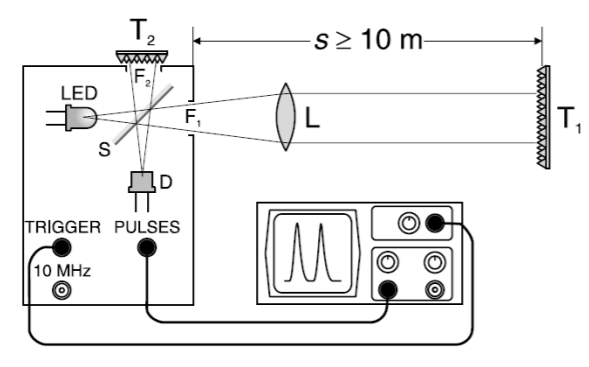
\includegraphics[width=6cm]{exp_1.png}
    \caption{Setup 1}
    \label{fig:setup1}
\end{figure}

For the second part of the experiment, we will use coaxial cables of various sizes. Coaxial cable is a type of transmission line used to transmit high frequency electrical signals with low losses, which is composed of an inner conductor surrounded by an isolating material which is itself surrounded by a conducting shield. Additionally we have an oscilloscope and a pulse generator.

\begin{figure}[h!]
    \centering
    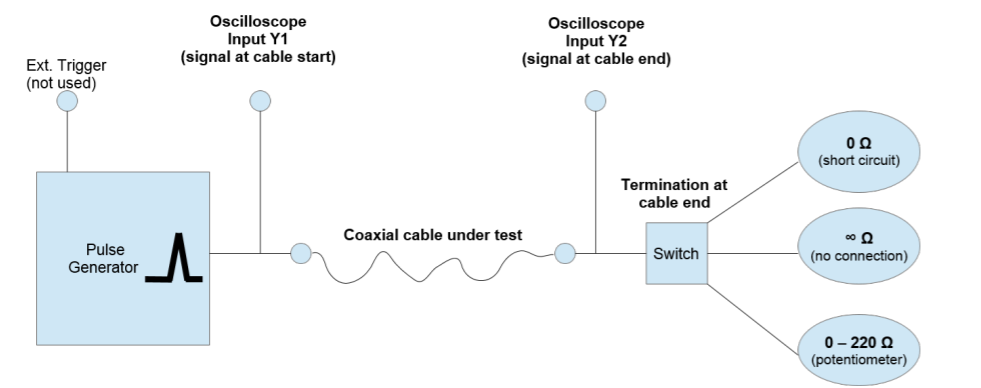
\includegraphics[width=8cm]{exp_2.png}
    \caption{Setup 2}
    \label{fig:setup2}
\end{figure}

\section{Results}

\subsection{Measuring the speed of light in air}
In order to determine the speed of light in air for the first part of our experiment, we measure the time the light takes to travel a certain distance, that means the time it takes to be reflected by the mirror $T_1$ and back. We will measure the time for different distances and get the line graph (see Graph 1).
The reason for using the slope of that graph and not the individual values is because we don't know the exact total distance of the light, since the beam splitter and the detector are inside the box. That way we get a more accurate result.

\begin{figure}[ht]
\centering
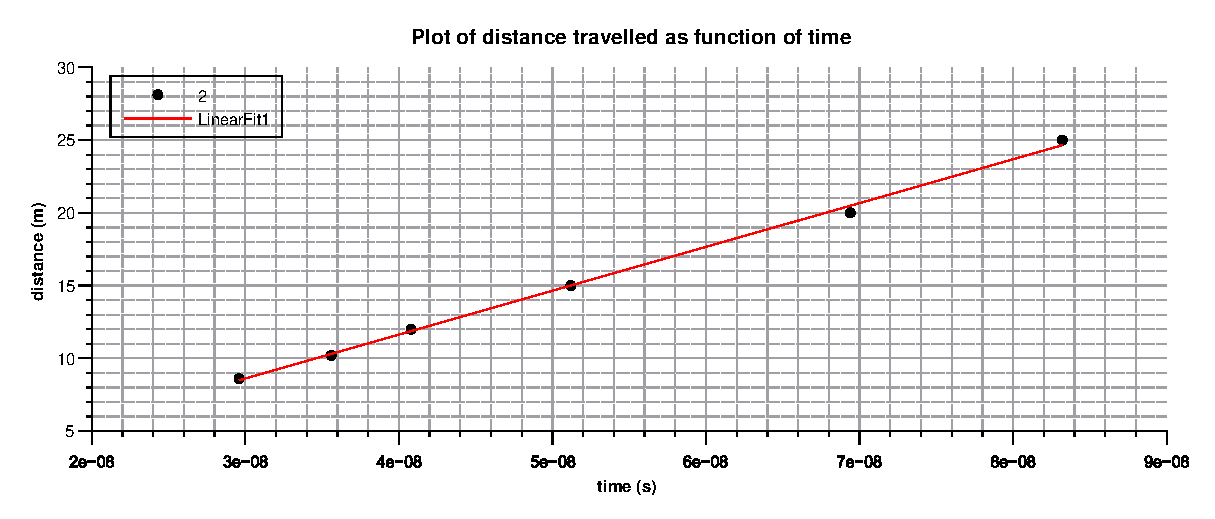
\includegraphics[width=13cm]{Graph1.eps}
\caption{Graph 1: The distance by light as function of time}
\label{fig:my_label}
\end{figure}

Since the speed of light is constant, we can use the relationship $x=ct$ and the slope of our linear fit to determine $c$: $\boxed{c_{exp} \approx 3,015 \cdot 10^8 m\cdot s^{-1}}$

\medskip

We can also determine the relative distance from the fixed value of c:

\begin{center}
$\frac{\vert c - c_{exp}\vert}{c}\cdot 100 \approx 0.6\%$
\end{center}

\subsection{Measuring the speed of light in a coaxial cable}

    To measure the speed of light in a coaxial cable we have to measure the time $\Delta{t}$ the electromagnetic wave takes for 4 reflections (sometimes 3) in function of the length of the cable. We measure the time $\Delta{t}$ directly on the oscilloscope, the 4 reflections represented by 4 peeks, which means the pulse travels 12 times the distance of the cable, but when the cable exceeds $100m$, only 3 peeks are visible. We should note that only the signal at the cable start (input 1) worked on our oscilloscope. Channel 2 didn't show any signal. We collected our results in a graph (see Figure(4)) and displayed the linear fit of the function.
    Using the relation: $t=\frac{1}{c_{coax}}\cdot{d}$, we get:

\begin{equation}
    c_{coax} \approx 2,05\cdot 10^8 \ m\cdot s^{-1} \approx \frac{2}{3}c_0
\end{equation}

\begin{figure}
    \centering
    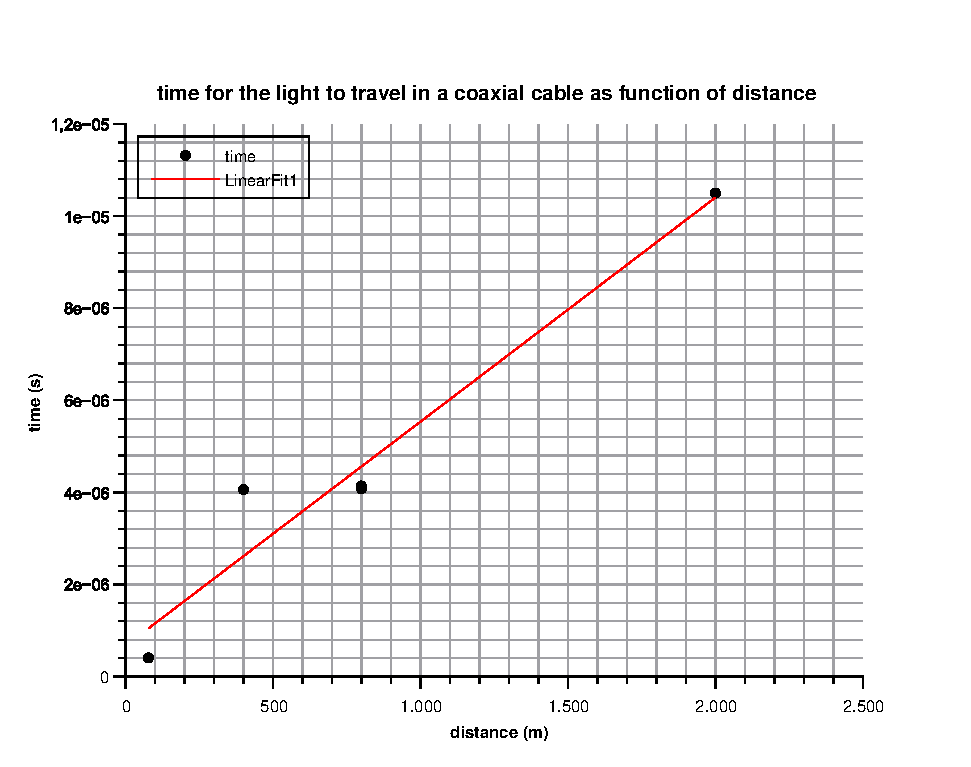
\includegraphics[width=10cm]{Graph2.eps}
    \caption{Graph 2: time for the light to travel through the cable as function of distance}
    \label{fig:my_label}
\end{figure}

\subsection{Measuring the Inductance, Capacity and Impedance}
For this last part of the experiment, we want to measure the inductance and capacity per unit length $L^*$ and $C^*$ respectively. As we know from the handout, the magnetic permeability $\mu=1$ and $\mu_0=4\pi\cdot{10^{-7}}H.m^{-1}$. In order to find the dieletric constant $\varepsilon$ we simply use this relation with our results found previously:

\begin{equation}
    c_{coax}=\frac{c_0}{\sqrt{\varepsilon}} 
\end{equation}

We obtain $\varepsilon= (\frac{c_0}{c_{coax}})^2\approx 2.14$ and know that $\varepsilon_0=8,854\cdot{10^{-12}F.m^{-1}}$.
\newline
We measure the radius of the inner conductor and get $r_1=0,35mm$ and the insulation layer $r_2=1,0mm$.
We can now calculate the inductance and capacity given by these equations:

\begin{equation}
    L^*=\frac{\mu_0\mu}{2\pi}\cdot{\ln\frac{r_2}{r_1}}= 2,1\cdot{10^{-7}}H/m
    \hspace{1cm} and \hspace{1cm}
    C^*=\frac{2\pi\varepsilon_0\varepsilon}{\ln\frac{r_2}{r_1}} \approx 1,13 \cdot{10^{-10}} \ F\cdot m^{-1}
\end{equation}

With these results, we can finally calculate the impedance of the coaxial cable.
\begin{equation}
    Z_c=\sqrt{\frac{L^*}{C^*}} \approx 43,1 \ \Omega
\end{equation}
The termination at the cable end had three different option. The first one, $0\Omega$, meaning that it is a short circuit, was used for all our measurements. Then we have an open circuit, represented on the switch by $\infty \Omega$, made still reflections of the signal but there was no polarization. Finally, using the potentiometer we can measure the impedance of the cable again. 

\centering
\begin{tabular}{|c|c|}
    \hline
    cable \ length \ (m) & measured \ impedance \ ($\Omega$) \\
    \hline
    33 & 55 \\
    \hline
    66.66 & 50.6 \\
    \hline
    100 & 52.8 \\
    \hline
\end{tabular}
\flushleft

\begin{equation}
    \boxed{\Rightarrow Z_{avg} = 52.8 \Omega}
\end{equation}

\subsubsection{Theoretical capacitance}

    \begin{equation}
        Gauss\ Law : \ \iint_{\partial V}\vec{E}\cdot d\vec{S} = \frac{1}{\varepsilon_r \varepsilon_0}\iiint_V \rho dV
    \end{equation}

    For symmetry reasons, the electrical field of the coaxial cable is only dependent on the radius $r$, if we consider cylindrical coordinates: $\vec{E}(r,\phi,z) = \vec{E}(r) = E_r\vec{e_r}$. Using Gauß' Law we can then determine $E_r$
    
    \begin{equation}
        \iint_{\partial V}E_r(r)rd\phi dz = \frac{\rho}{\varepsilon_r\varepsilon_0}\iiint_V rdrd\phi dz
    \end{equation}
    
    With following integration borders:
    
    \centering
    $
        0 \leq r \leq r_1 \\
        0 \leq \phi \leq 2 \pi \\
        0 \leq z \leq l 
    $

    \flushleft
    And where R is the radius of our arbitrarily chosen Gaussian surface, which we choose to be a cylinder.
    

    \begin{equation}
        E_r(r) \cdot 2\pi rl = \frac{\rho r_1^2 \pi l}{\varepsilon_r\varepsilon_0} 
    \end{equation}
    
    \begin{equation}
        \boxed{\Rightarrow \vec{E}(r) = \frac{\rho r_1^2}{2\varepsilon_r \varepsilon_0 R}\vec{e_r}}   
    \end{equation}
    
    We can now look at the potential:
    
    \begin{equation}
        \Phi = - \int_{r_1}^{r^2}\vec{E}(r)\cdot d\vec{r} 
    \end{equation}
        
    \begin{equation}
        \boxed{\Leftrightarrow \Phi = - \int_{r_1}^{r^2}\frac{\rho r_1^2}{2\varepsilon_R \varepsilon_0 r}dr = \frac{\rho r_1^2}{2\varepsilon_r \varepsilon_0} \ln {\frac{r_2}{r_1}}}  
    \end{equation}
    
    We also have the relation, for a homogeneous charge distribution $\rho$, $Q = \rho V$, where Q is the total charge and V the volume. In our case, this simply yields $\rho = \frac{Q}{\pi l r_1^2}$ 
    
    The capacitance can be destermined with the relation $C = \frac{Q}{\Phi}$
    
    \begin{equation}
        \Rightarrow C = \frac{2\pi l\varepsilon_r \varepsilon_0}{\ln{\frac{r_2}{r_1}}}
    \end{equation}
    
    \begin{equation}
        \boxed{\Rightarrow \frac{dC}{dl} = C^* = \frac{2\pi  \varepsilon_r\varepsilon_0}{\ln{\frac{r_2}{r_1}}}}
    \end{equation}

\subsubsection {Theoretical inductance}

\begin{figure}[h]
    \centering
    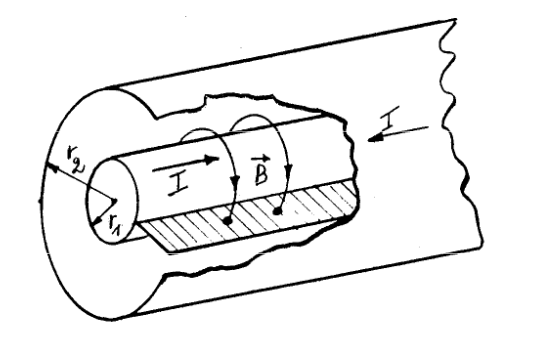
\includegraphics[width=8cm]{coaxial cable.PNG}
    \caption{Representation of a coaxial cable}
    \label{fig:my_label}
\end{figure}

\begin{equation}
    \oint_c {\vec{B}} d{\vec{l}} = \mu\mu_0 I_{en}
\end{equation}

\centering
$for \, \rho \geq r_1$, $I_{en} = I$ \qquad $for \, \rho < r_1$ , $I_{en}=I\frac{A_c}{A_{cyl}}=I\frac{\pi\rho^2}{\pi r_1^2}=\frac{\rho^2}{r_12}$
\flushleft



for a Circle C, the integral becomes
\begin{equation}
    \int_{\phi=0}^{2\pi}\vec{B}\cdot(\hat{\phi}\rho d\phi)=\mu\mu_0 I_{en}
\end{equation}

Since the current distribution is uniform and assumed infinite in the z-direction, $\vec{B}$ is independent of z $\Rightarrow \vec{B}\cdot \hat{z}=0$
The radial symmetry of the problem and the invariance for any amount of rotation in $\phi$ imply $\vec{B}(\rho,\phi,z)= B(\rho)\vec{e_{\phi}}$. So we get

\begin{equation}
    \mu\mu_0 I_{en}=\int_{\phi=0}^{2\pi}B(\rho)\hat{\phi}\cdot(\hat{\phi}\rho d\phi)
\end{equation}
\begin{equation}
     =\rho B(\rho) \int_{\phi=0}^{2\pi}d\rho = 2\pi \rho B(\rho)
\end{equation}

Which leads us to
\begin{equation}
   \boxed{\vec{B}=\frac{I\mu\mu_0}{2\pi \rho}\hat{\phi} \qquad for \, \rho \geq r_1}
\end{equation}
\begin{equation}
    \boxed{\vec{B}=\frac{I \mu\mu_0\rho}{2\pi r_1^2}\hat{\phi} \qquad for \, \rho < r_1}
\end{equation}


We know that the inductance is defined by
\begin{equation}
    L:= \frac{\Phi}{I}
\end{equation}
where $\Phi$ is the magnetic flux, which we get by integrating over the magnetic flux density over an arbitrary open surface \textbf{\textit{S}} trough which all magnetic field lines must pass.
\begin{equation}
    \Phi =\iint_{\textbf{\textit{S}}}\vec{B}\cdot d\vec{s}
\end{equation}
With a plane of constant $\phi$, length \textbf{l}, perpendicular to the magnetic field lines we get
\begin{equation}
    \Phi = \int_{\rho=r_1}^{r_2}\int_{z=0}^{l}(\frac{\mu\mu_0 I}{2\pi \rho}\hat{\phi})\cdot(\hat{\phi}d\rho dz)
\end{equation}
\begin{equation}
    =\frac{\mu\mu_0 I}{2\pi}\int_{z=0}^{l}dz\int_{\rho=r_1}^{r_2}\frac{d\rho}{\rho}
\end{equation}
\begin{equation}
   \boxed{\Rightarrow \Phi =\frac{\mu\mu_0 I l }{2\pi}\ln{\frac{r_2}{r_1}}}
\end{equation}

And finally we get
\begin{equation}
    L:=\frac{\Phi}{I} =\frac{\frac{\mu\mu_0 I l}{2\pi}\ln{\frac{r_2}{r_1}}}{I}
\end{equation}
\begin{equation}
    \boxed{\Rightarrow L= \frac{\mu\mu_0 l}{2\pi}\ln{\frac{r_2}{r_1}}}
\end{equation}
Which gives us the inductance per unit of length L*
\begin{equation}
    \boxed{L*=\frac{\mu\mu_0}{2\pi}\ln{\frac{r_2}{r_1}}}
\end{equation}

\section{Conclusion}

In this experiment we were able to determine the speed of light in different media. In the first part we measured a value of $c_{air}\approx3,015\cdot10^8m s^{-1}$ for the speed of light in air, which would surpass the speed of light in vacuum $c_0$, which we know is not possible. The deviation of about $0,6\%$ from $c_0$ is however well within the measurement inaccuracy of the experimental setup. We can therefore still conclude that air as a medium does not have a great effect on the speed of light. In the second part of the experiment we determined the speed of light in a coaxial cable to be $c_{coax}\approx2,05\cdot10^8ms^{-1}$ which equals approximately $\frac{2}{3}c_0$. We can thus conclude that the coaxial cable has a greater effect on the propagation speed of electromagnetic waves.
The third part of the experiment was dedicated to the determination of the impedance of the coaxial cable. Here we obtained a theoretical value of $Z_c\approx43,1 \Omega$, from which our experimentally determined value of $Z_{avg}=52.8 \Omega $ deviates by 22.5\%.


\end{document}



